\section{Objectives}

\subsection{Main Objective}

The main objective of this project is to generate a black and white composite
video signal that will drive a Cathode Ray Tube (CRT) television. To accomplish
this, we will develop a video card with a serial interface that can generate a
composite video signal. We will be able to achieve a resolution of 240 x 320
pixels on the screen.

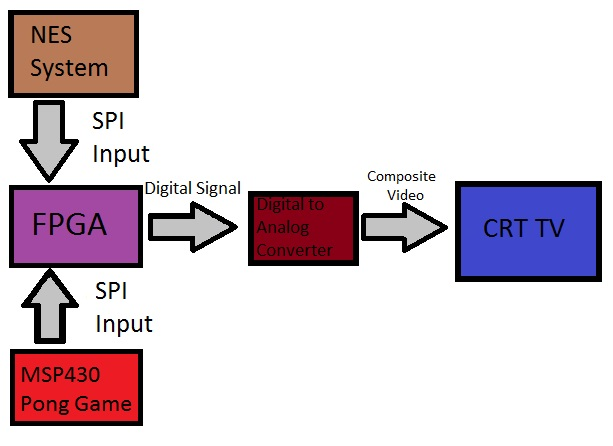
\includegraphics{Diagram}
\begin{figure}[H]
   \centering
   \caption{System Overview}
\end{figure}

\subsection{Secondary Objectives}

\subsubsection{Framerate Control}

The framerate for a CRT is roughly 30Hz while the shutter rate for most video
cameras is 24Hz. When filming a CRT screen, slightly more than one frame will be
displayed in the time that the image is captured on the camera, this results in
a sweeping, white bar that will appear on the television when viewing the film.
This is undesireable.

Many prosumer and professional cameras have an output signal called HSYNC. This
signal will be used to trigger the composite video encoder so that only one
frame is written to the television during one shutter period. In theory this
will remove any erronous artifacts that would normally be seen in the video.

\subsubsection{Sound Synthesizer}

Adding to the SPI interface, we could add commands that trigger pre-generated
sound "bites" which would play in conjunction with pong. These sounds could
either be programmed to the encoder through SPI, and saved into RAM or hardcoded
into ROM. A DAC would then be needed to drive a speaker. Sound information and
playing would be modeled after some standard, possibly something like WAV.

\subsubsection{Open MSP430 Synthesis}

On Opencores.com an open source IP of the MSP430 core can be downloaded for
synthesis in an FPGA. To cut back on the hardware used in the project, we can
put this core on our FPGA and program pong onto it. This also adds some
complexity as the ADC on the evaluation board would need to be interfaced to the
system.

\subsubsection{Colour}

The colour component of a composite signal is transmitted through the phase and
angle modulation of a 3.58MHz carrier. In order to generate this signal we would
need to employ a parallel DAC instead of our cheap, lopsided, but inexpensive
resistor divider DAC. Another project within our class is to create a Ninstendo
Entertainment System on an FPGA, and so we will base our colour output on the
NES.


\subsection{Hardware}

To be able to complete this project we will need more hardware than what we 
currently have. We have a MSP430 microcontroller, the FPGA board, and a mini
black and white TV. We need an 8-bit parallel, single channel DAC. We will use
the AD9748 from Analog Devices Inc. which can be ordered from Digikey, and we
will also need a breakout board for the 32-QFN package which can also be picked
up from Digikey. Any hardware we may need, such as parts for filtering will be
provided by us.
